\iffalse
This file is protected by Copyright. Please refer to the COPYRIGHT file
distributed with this source distribution.

This file is part of OpenCPI <http://www.opencpi.org>

OpenCPI is free software: you can redistribute it and/or modify it under the
terms of the GNU Lesser General Public License as published by the Free Software
Foundation, either version 3 of the License, or (at your option) any later
version.

OpenCPI is distributed in the hope that it will be useful, but WITHOUT ANY
WARRANTY; without even the implied warranty of MERCHANTABILITY or FITNESS FOR A
PARTICULAR PURPOSE. See the GNU Lesser General Public License for more details.

You should have received a copy of the GNU Lesser General Public License along
with this program. If not, see <http://www.gnu.org/licenses/>.
\fi

%----------------------------------------------------------------------------------------
% Update the docTitle and docVersion per document
%----------------------------------------------------------------------------------------
\def\docTitle{OpenCPI\\ Matchstiq-Z1 Getting Started Guide}
\def\docVersion{1.3}
%----------------------------------------------------------------------------------------
\input{../../../../../../doc/av/tex/snippets/LaTeX_Header.tex}
\date{Version \docVersion} % Force date to be blank and override date with version
\title{\docTitle}
\lhead{Matchstiq-Z1 Getting Started Guide}
%----------------------------------------------------------------------------------------
\usepackage[T1]{fontenc} % http://tex.stackexchange.com/a/181119
\usepackage{graphicx}
\graphicspath{ {figures/} }
\usepackage{textcomp}
\begin{document}
\maketitle
%\thispagestyle{fancy}
\newpage

	\begin{center}
	\textit{\textbf{Revision History}}
		\begin{table}[H]
		\label{table:revisions} % Add "[H]" to force placement of table
			\begin{tabularx}{\textwidth}{|c|X|l|}
			\hline
			\rowcolor{blue}
			\textbf{Revision} & \textbf{Description of Change} & \textbf{Date} \\
		    \hline
            v1.1 & Initial Release & 3/2017 \\
            \hline
            v1.2 & Updated for OpenCPI Release 1.2 & 8/2017 \\
            \hline
            v1.3 & Updated for OpenCPI Release 1.3 & 2/2018 \\
            \hline
			\end{tabularx}
		\end{table}
	\end{center}

\newpage

\tableofcontents

\newpage

\section{References}

	This document assumes a basic understanding of the Linux command line (or ``shell'') environment.  The reference(s) in Table 1 can be used as an overview of OpenCPI and may prove useful.

\def\refcapbottom{}
\input{../../../../../../doc/av/tex/snippets/References_Table}

\newpage
\section{Overview}
This purpose of this document is to allow the user to install OpenCPI on the Matchstiq-Z1 SDR.  The software platform on the Matchstiq is the same as the software platform for the ZedBoard. This means several of the files that are used to create the Matchstiq-Z1 SD card come from the ZedBoard SD card.
\section{Prerequisites}
\begin{flushleft}
This guide assumes that the following RPMs are installed:  \\
\begin{table}[H]

		\label{table:rpms}
			\begin{tabularx}{\textwidth}{|c|X|}
			\hline
			\rowcolor{blue}
			\textbf{RPM Name} & \textbf{Description} \\
			\hline
			All prerequisite RPMs & These packages have OpenCPI-specific patches and are provided as RPMs. This packaging ensures they will not conflict with other installed copies by using a nonstandard installation location of \path{/opt/opencpi/prerequisites}. \\
				\hline
				\small{\code{opencpi-*.x86\_64.rpm}} &
								Base installation RPM includes the runtime portion of the Component Development Kit (CDK), scripts for creating the user's workspace, limited documentation, and a read-only \code{ocpi.core} Project containing framework essential components, workers, platforms, etc. \\
				\hline
				\small{\code{opencpi-devel-*.x86\_64.rpm}} &
				Additional header files and scripts for developing new assets as HDL and/or RCC. \\
				\hline
				\small{\code{opencpi-hw-platform-zed-*.noarch.rpm}} &
				Additional files necessary to build the framework targeting specific hardware platforms. Automatically requires the zed sw-platform package. \\
				\hline
				\small{\code{opencpi-project-assets*.noarch.rpm}} &
				The \texttt{ocpi.assets} Project, which contains the remaining supported OpenCPI resources, e.g. additional Platform Support, Workers, Demo Applications, etc. \\
				\hline
				\small{\code{opencpi-sw-platform-xilinx13\_3-*.noarch.rpm}} &
				Additional files necessary to build the framework targeting the xilinx13\_3 software platform. \\
				\hline
			\end{tabularx}
\end{table}
This guide assumes that the Core and Assets projects have user copies and have been registered. Creating user copies of projects is done by using the new\_project\_source script as described in the Getting Started Guide.  registering projects is done by running the command \code{ocpidev register project} at the top level of the project.   \\ \bigskip

The SDR that is expected to be used is the Epiq Matchstiq-Z1 (ensure you are using the Z1 version).  A USB to Ethernet adapter will need to be plugged in to the front panel micro-USB port.  The SDR gets an IP Address by using DHCP.  It is a requirement if operating in network mode (discussed later) that the USB to Ethernet adapter is connected to a network that uses DHCP\footnote{Static IP addresses are possible but have not been integrated with the OpenCPI startup procedure at this time.}. \\ \bigskip

There is a micro-USB serial port on the back of the SDR; to expose this port, the two screws in the back plate need to be removed.  A Male micro-USB cable will need to be plugged into this port to access the serial connection.  On some versions of the Matchstiq-Z1, \textit{this connector can be very fragile}, \textbf{so be careful}.\\ \bigskip

\begin{figure}[ht]
	\centerline{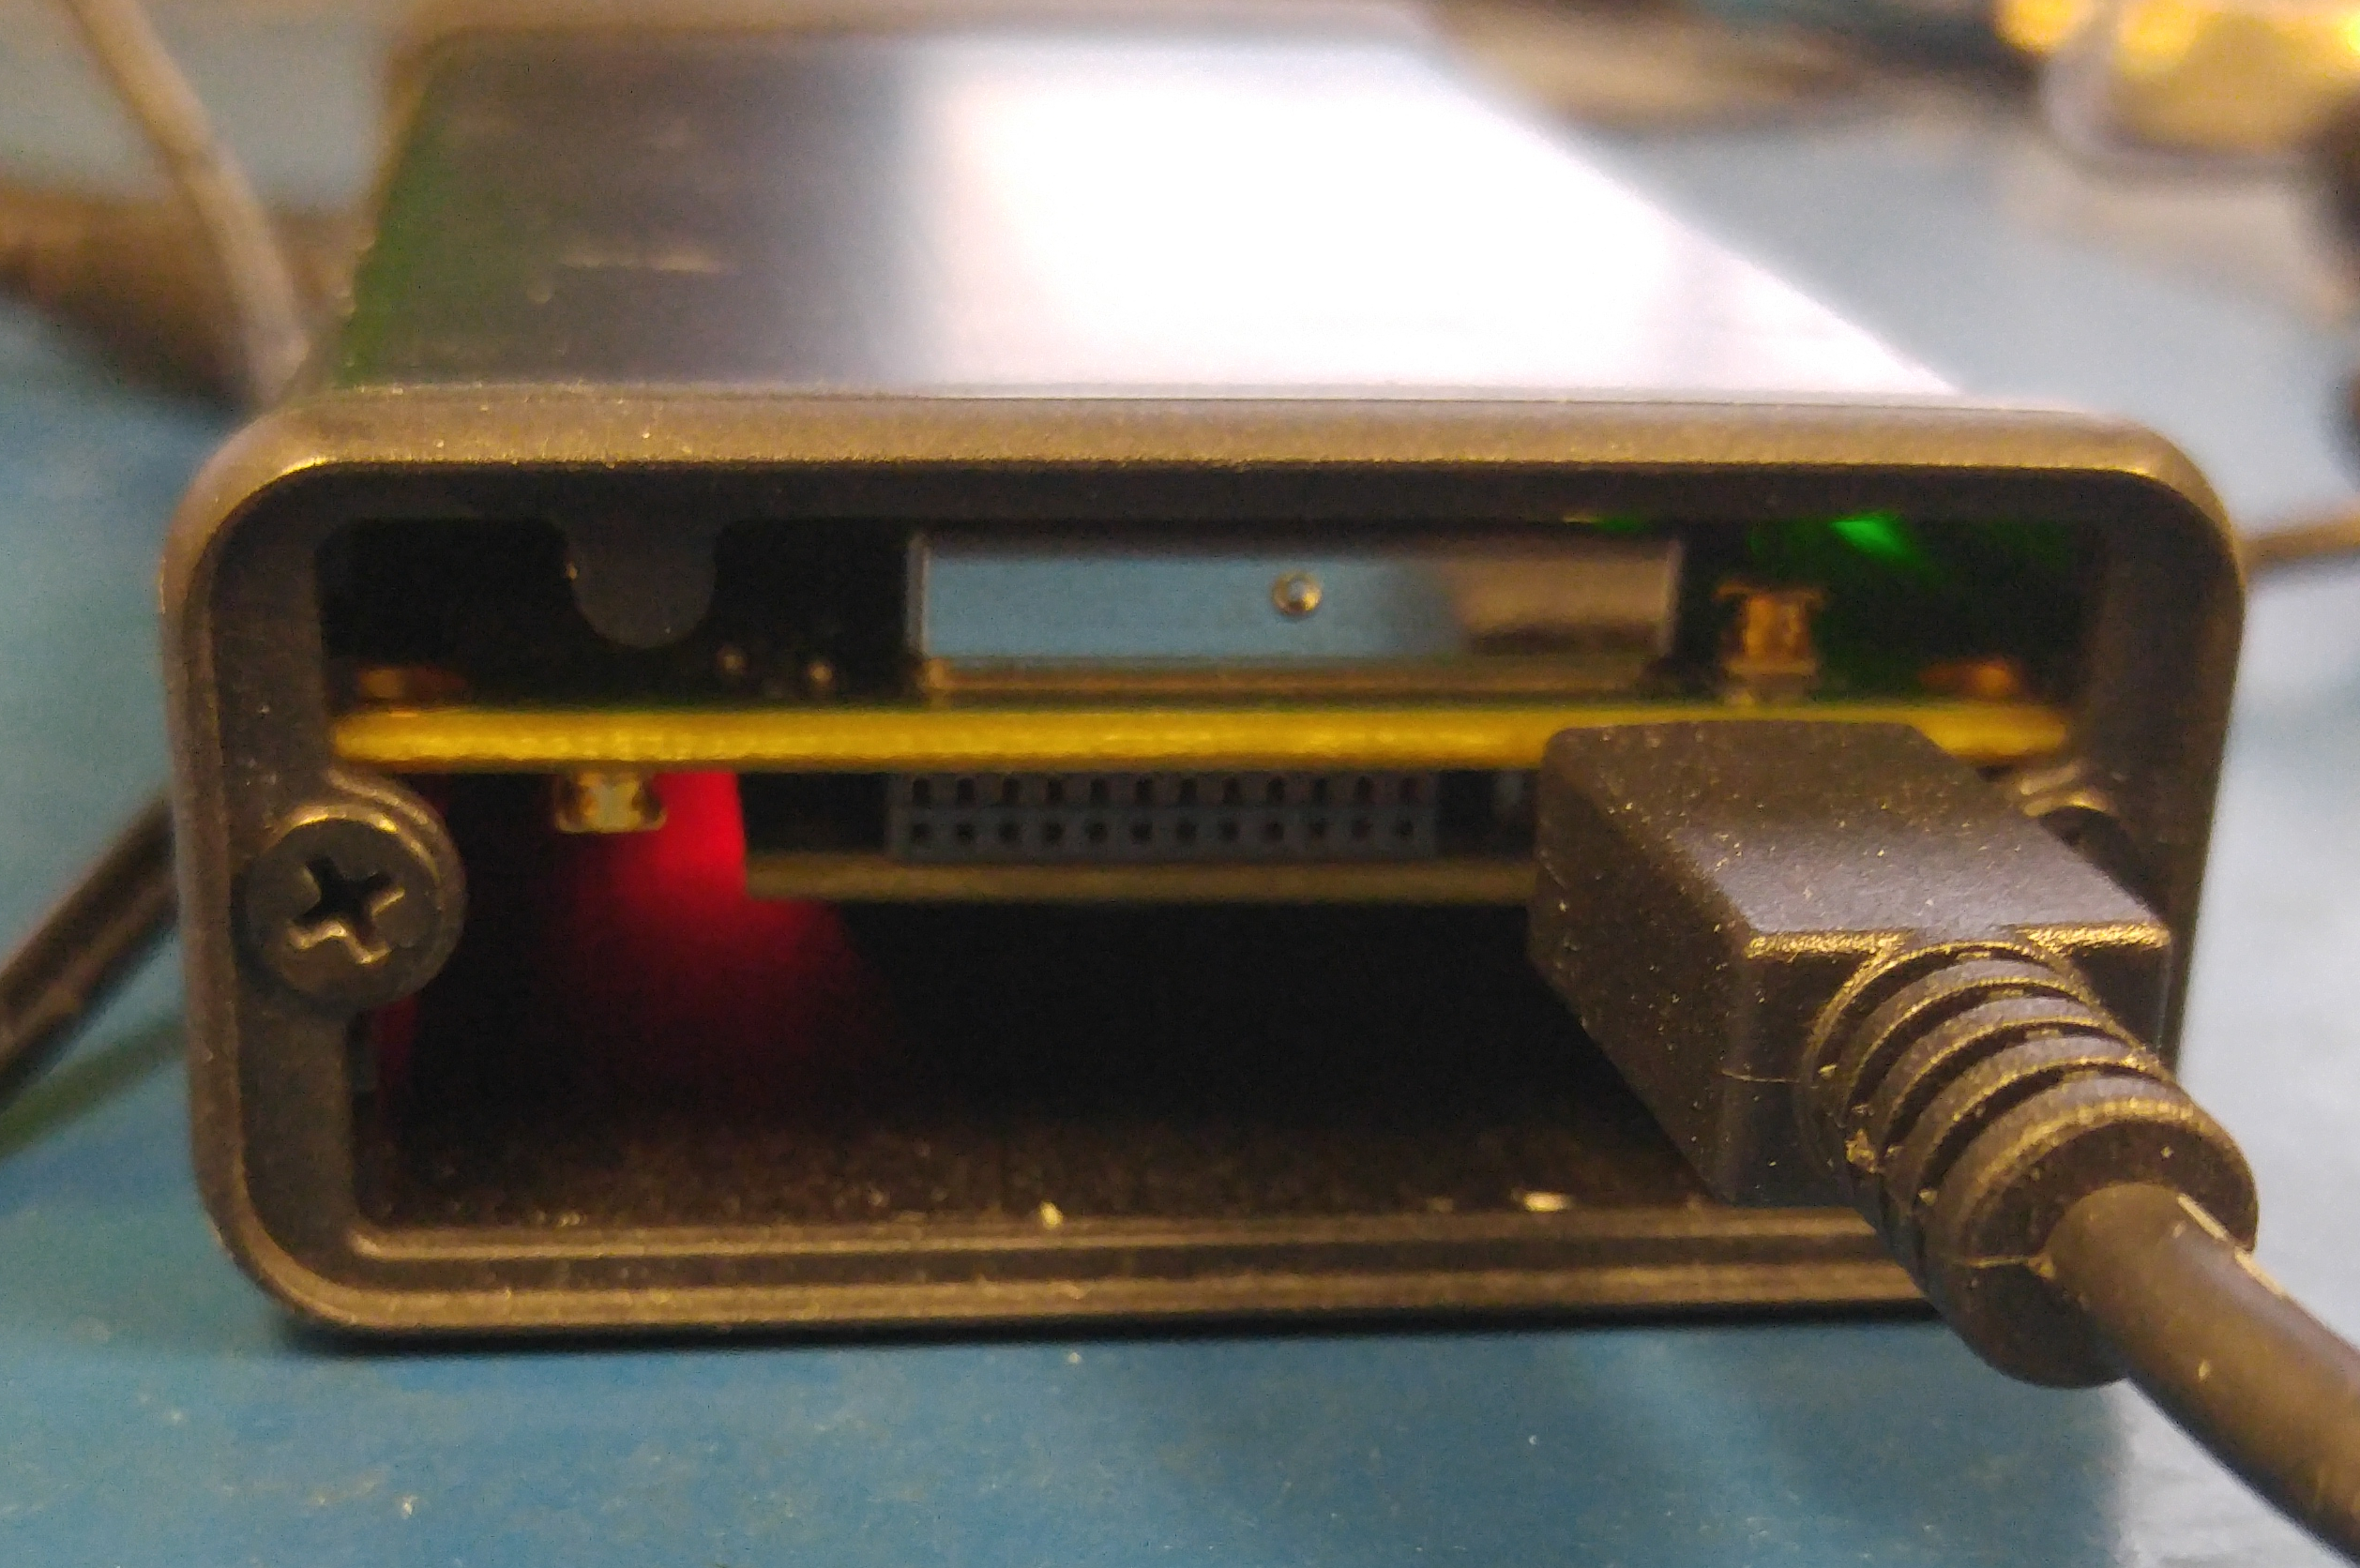
\includegraphics[scale=0.08]{Matchstiq_Z1_backpannel}}
	\caption{Connected Back Panel}
	\label{fig:back}
\end{figure}

On the front panel of the SDR, there are three labeled SMB (50 Ohm) connectors. One each for Receive (RX), Transmit(TX), and GPS.  The SDR comes with 2 SMB to SMA adapters.  This means that any RF cabling should use SMA or SMB connectors and be rated up to at least 3GHz which is the maximum TX/RX frequency of the radio. \\   \bigskip
\begin{figure}[ht]
	\centerline{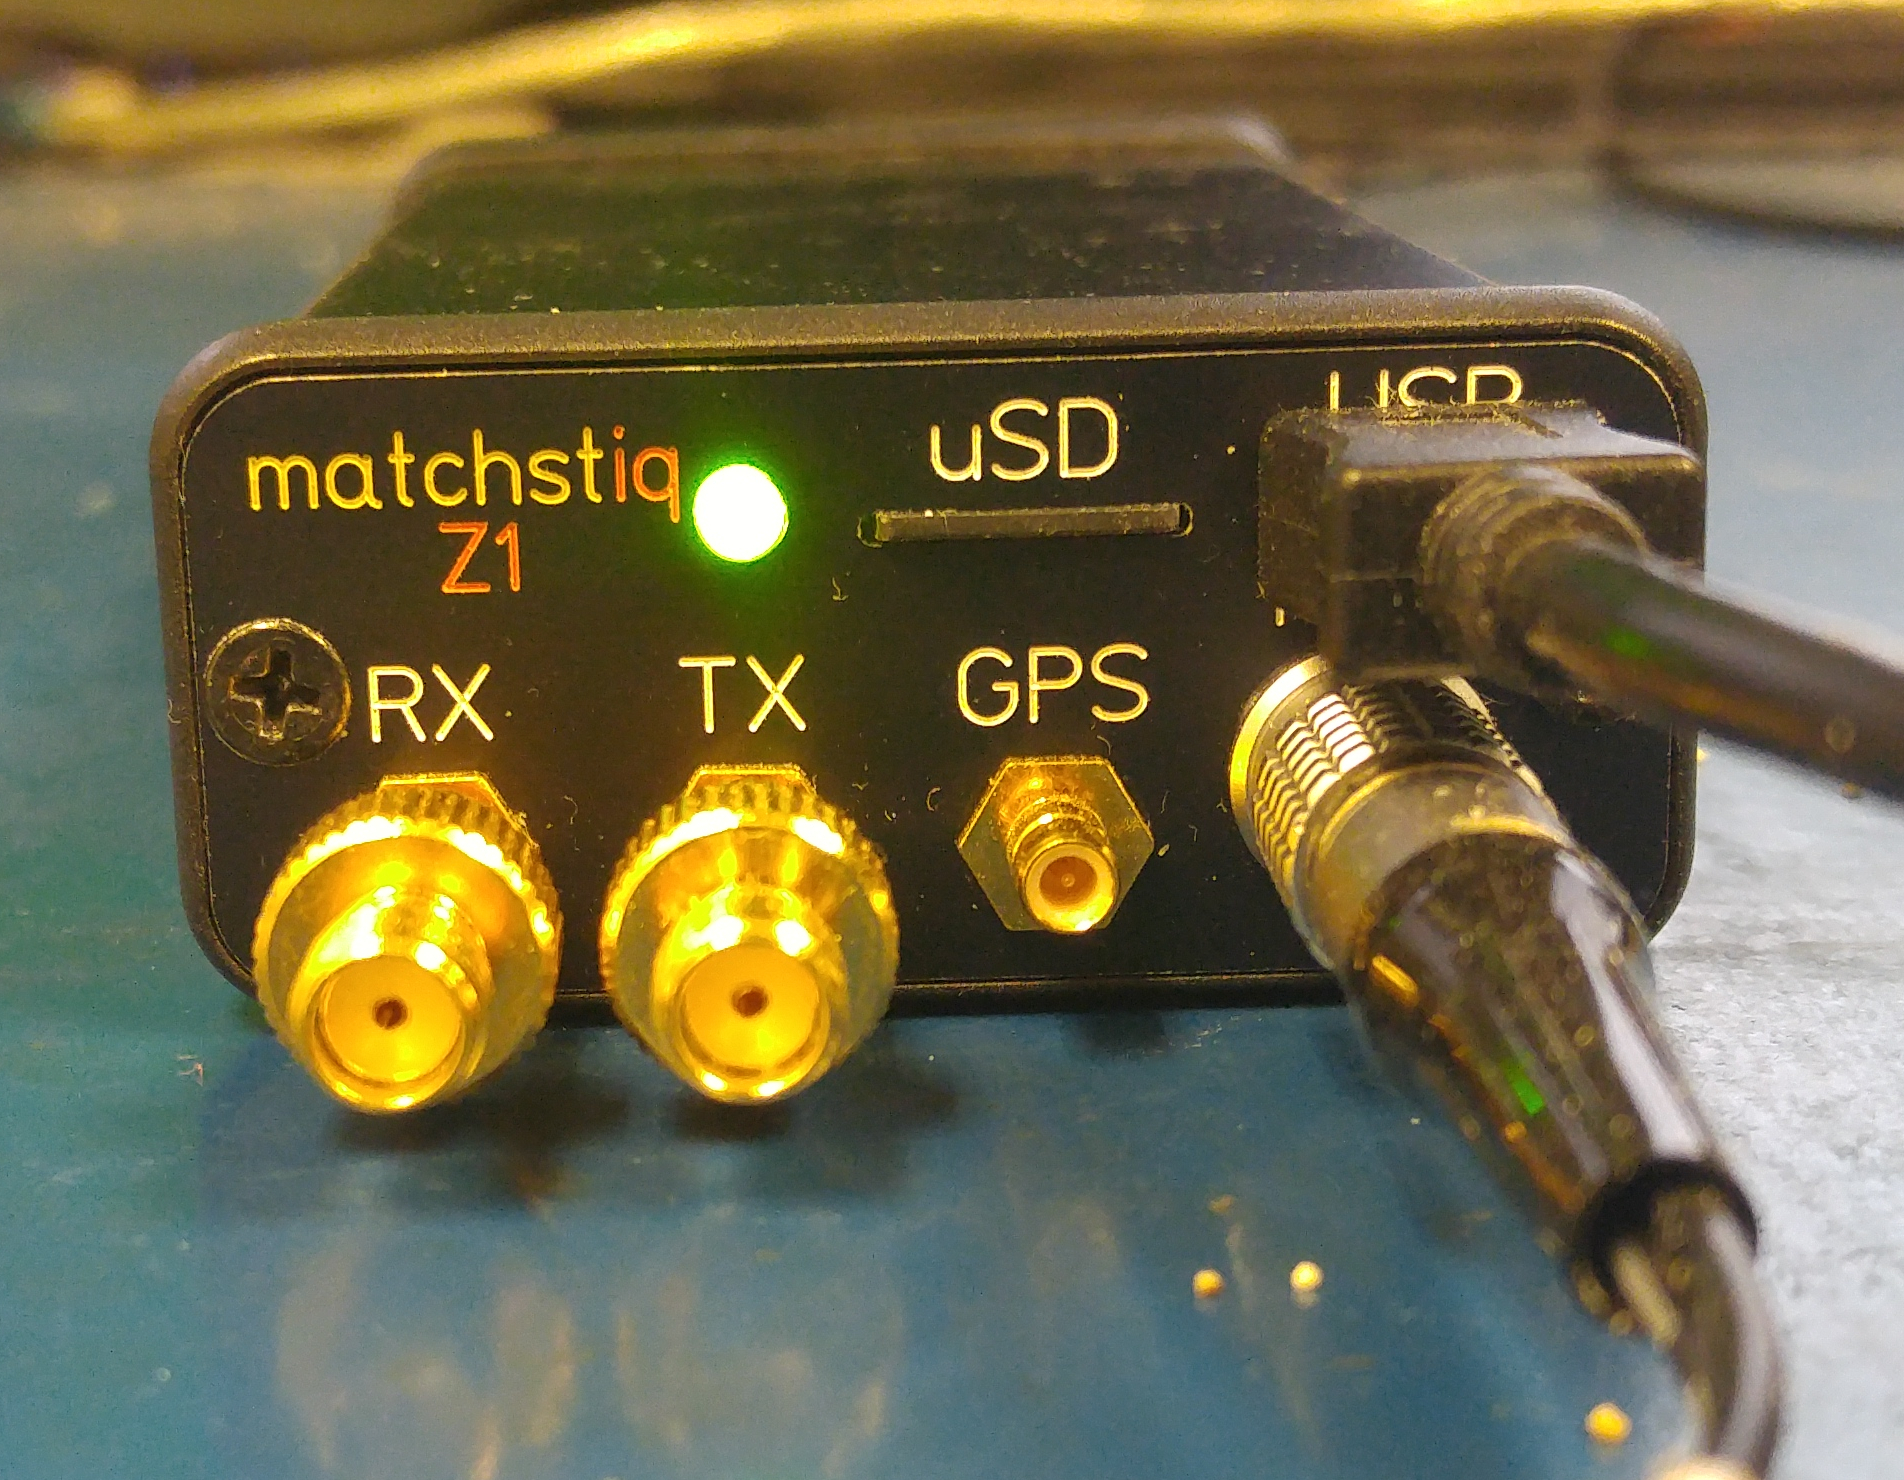
\includegraphics[scale=0.1]{Matchstiq_Z1_frontpannel}}
	\caption{Connected Front Panel}
	\label{fig:front}
\end{figure}
\end{flushleft}

\section{Script Setup}
There are two modes for running applications on any embedded radio: network mode and standalone mode.  Network mode is when the development system hosts the OpenCPI tree as an NFS server to the Matchstiq-Z1 as an NFS client.  This configuration provides easy and dynamic access to all of OpenCPI, and presumably any components and applications.  Standalone mode is when all the artifacts are located on the SDR's local storage (\textit{e.g.} SD card) and no network connection is required.  This is a better \textit{deployment} mode, and is better for situations where a network connection is not possible or practical.  Network mode is generally preferred when it is possible because it makes the development process easier than standalone mode.

\begin{flushleft}
For each mode, there are separate startup scripts that are run on the SDR. These scripts will need to be modified for each user's specific setup and file structure.  There are starting points for these scripts that are provided by the framework.  For networked mode the script is located at \path{/opt/opencpi/boot_support/zed/OpenCPI-SD-zed/opencpi/default_mynetsetup.sh}.  For standalone mode, the script is located at \path{/opt/opencpi/boot_support/zed/OpenCPI-SD-zed/opencpi/default_mysetup.sh}.  These scripts need to be renamed to \texttt{mynetsetup.sh} and \texttt{mysetup.sh} before they are copied over to the SD card in Section \ref{sec:HW_Setup}. \\ \bigskip

\textit{For either usage mode}, the following settings that are passed by \texttt{mynetsetup.sh/mysetup.sh} to the \texttt{zynq\_net\_setup.sh/zynq\_setup.sh} scripts \textit{might} need to be modified:
\end{flushleft}

\begin{itemize}
 \item The system to be used as a time server. Defaulted to ``time.nist.gov''. Change this if you have a local time sever that supports RFC-868.
 \item The current timezone description. Defaulted to ``EST5EDT,M3.2.0,M11.1.0''.  Change this if required for the local timezone. See \texttt{man tzset} on the host PC for more information.
 \item If you do not have a time server, or cannot connect to a time server, you will need to manually set the time at start up.  Use the date command to manually set the Linux system time. See \texttt{man date} on the host PC for more information.  If Linux system time is not required to be accurate, you can skip this step.
\end{itemize}

\begin{flushleft}
\textit{When using Network Mode}, the following modifications are required:
\end{flushleft}

\begin{enumerate}
\item In \texttt{mynetsetup.sh}, find the following lines which are necessary for mounting Assets Project and the Core Project:
\begin{verbatim}
mkdir -p /mnt/ocpi_core
mount -t nfs -o udp,nolock,soft,intr $1:/home/user/ocpiCore /mnt/ocpi_core
mkdir -p /mnt/ocpi_assets
mount -t nfs -o udp,nolock,soft,intr $1:/home/user/ocpiAssets /mnt/ocpi_assets
\end{verbatim}
 \item Edit \texttt{/home/user/ocpiCore} and \texttt{/home/user/ocpiAssets} to reflect the paths to the Core Project and Assets Project on the host.
\end{enumerate}
\begin{flushleft}
\label{sec:buildNow}
\textit{For Standalone Mode}, all OpenCPI artifacts required to run any applications on the SDR need to be copied onto the SD card.  So, you must build these artifacts earlier when operating in Standalone Mode. Perform the steps in Section \ref{sec:buildverify}  now. The artifacts created will be copied over to the SD card in Section \ref{sec:HW_Setup}. In general, you will want to copy any required \texttt{.so} (RCC workers), \texttt{.bit.gz} (hdl assemblies), and application XMLs or executables into the ATLAS partition of the SD card.
\end{flushleft}
\section{Hardware and SD Card Setup}
\label{sec:HW_Setup}
The Matchstiq-Z1 SDR is equipped with two SD card slots: one internal and one accessible via the front panel. The SDRs are shipped from Epiq Solutions with an SD card installed in the internal slot that is loaded with their embedded environment. However, when an SD card is installed in the front panel SD slot, the SDR will choose to operate from this SD card rather than the internal SD card. Therefore, a user can easily switch the SDR between operating in the Epiq or AV environments.
\begin{flushleft}
Since the internal SD card is already formatted correctly, this guide assumes it has been removed for use in the front panel slot. If you wish to use your own SD card, you must ensure that it is formatted correctly. To gain access to the internal SD card slot, remove the screws from the front and back plates of the SDR and slide the board assembly out of the enclosure. Flip the SD card slot open and lift the card out.
\end{flushleft}
\subsection*{Make a backup image of iVeia SD card (assumes Linux host)}
\begin{itemize}
\item Determine the device file name for the SD card. It will likely be something like \texttt{/dev/sdb} or \texttt{/dev/mmcblk0}. To do this, you can take a look at the end of dmesg: ``\texttt{dmesg | tail -n 15}''.
\item Run the command ``\texttt{dd if=DEVICENAME of=backup.image}'' where DEVICENAME was determined above. This step should take $\sim15$ minutes depending on the card size.
\end{itemize}
\noindent To restore the card back to the original contents, run the command ``\texttt{dd of=DEVICENAME if=backup.image}'' (Do not do this step unless you want the original contents back on the SD card.)
\subsection*{Change boot files on the ``ATLAS'' partition}
All files except \texttt{u-boot.bin} can be ignored or deleted. Any files/directories copied to the ``ATLAS'' partition will appear at \texttt{/mnt/card} on the Matchstiq-Z1.
\begin{itemize}
\begin{minipage}{\linewidth}
\item Copy the following files/directories onto this partition:
\begin{itemize}
\item The entire folder \path{/opt/opencpi/boot_support/zed/OpenCPI-SD-zed/opencpi}
\subitem Remove from the SD card \path{opencpi/artifacts/*.bitz}
\item \path{/opt/opencpi/boot_support/zed/OpenCPI-SD-zed/uImage}
\item \path{/opt/opencpi/boot_support/zed/OpenCPI-SD-zed/uramdisk.image.gz}
\item \path{<Assets Project>/hdl/platforms/matchstiq_z1/sd_card/iveia-atlas-i-z7e.dtb}\footnote{This is the ZedBoard device tree with minor changes for Matchstiq-Z1.}
\end{itemize}
\item Copy the following files into the \texttt{opencpi} directory on this partition:
\begin{itemize}
\item \path{ocpiassets/hdl/platforms/matchstiq_z1/sd_card/system.xml}
\end{itemize}
\end{minipage}
\end{itemize}
\newpage
\subsection*{Copy the files needed for Standalone Mode to the ``ATLAS'' partition}
\textit{For Standalone Mode}:
\begin{itemize}
\begin{minipage}{\linewidth}
 \item Copy the following files into the \texttt{opencpi/xml} directory on this partition:
 \begin{itemize}
   \item \path{<Assets Project>/applications/bias.xml}
   \item \path{<Aseets Project>/applications/test.input}
 \end{itemize}
 \item Copy the following files into the \texttt{opencpi/artifacts} directory on this partition:
 \begin{itemize}
   \item \path{<Assets Project>/hdl/assemblies/testbias/container-testbias_matchstiq_z1_base/target-zynq/testbias_matchstiq_z1_base.bit.gz}
 \end{itemize}
\end{minipage}
\end{itemize}

\newpage
\begin{flushleft}
The SD card file structure should be as follows when these steps have been completed (ellipsis used to denote repetitive files):
\end{flushleft}
\begin{verbatim}
+-- iveia-atlas-i-z7e.dtb
+-- opencpi
|   +-- artifacts
|   |   +-- 001-bias_cc_s.so
       ...
|   |   +-- 020-testzc_s.so
|   |   \-- testbias_matchstiq_z1_base.bit.gz # only in Standalone Mode
|   +-- bin
|   |   +-- ocpibootstrap.sh
|   |   +-- ocpidriver
|   |   +-- ocpihdl
|   |   +-- ocpi_linux_driver
|   |   +-- ocpirun
|   |   +-- ocpiserve
|   |   +-- ocpixml
|   |   \-- ocpizynq
|   +-- lib
|   |   \-- linux-x13_3-arm
|   |       +-- libocpi_application_s.so
           ...
|   |       +-- libocpi_util_s.so
|   |       +-- mdev-opencpi.rules
|   |       \-- opencpi-3.10.0-xilinx-dirty-v14.7.ko
|   +-- mynetsetup.sh
|   +-- mysetup.sh
|   +-- system.xml
|   +-- xml
|   |   +-- bias.xml
       ...
|   |   +-- testbias.xml
|   |   +-- test.input # only in Standalone Mode
|   |   \-- time_test.xml
|   +-- zynq_net_setup.sh
|   \-- zynq_setup.sh
+-- u-boot.bin
+-- uImage
\-- uramdisk.image.gz
\end{verbatim}
\subsection*{No changes required for ``SDHOME'' partition}
All the files in this partition can be ignored. If space for files is required for your application, they can be deleted.
\subsection*{Serial setup}
By default, the USB to serial adapter will connect as read-only unless \texttt{udev} rules are added to have the device connect as read write.  Copy the file from the Assets Project \path{hdl/platforms/matchstiq_z1/97-matchstiq_z1.rules} to \path{/etc/udev/rules.d/}.  This will cause the USB to Serial adapter to connect as \texttt{/dev/matchstiq\_z1\_0} with read and write permissions for all users.  To connect to the serial port use the command ``\texttt{screen /dev/matchstiq\_z1\_0 115200}''.
\subsection*{Update U-Boot variables}
\begin{enumerate}
\item Remove power from the Matchstiq-Z1 unit.
\item Insert the SD card into the front panel SD card slot.
\item Connect a terminal to the rear micro-USB connector of the Matchstiq-Z1 with a baud rate of 115200.
\begin{itemize}
\item per the previous section, ``\texttt{screen /dev/matchstiq\_z1\_0 115200}'' can be used to connect to the serial port.
\end{itemize}
\item Apply power to the Matchstiq-Z1 with the terminal still connected and stop the boot process by hitting any key to enter the U-Boot terminal.
\item Run the following commands to setup the environment variables:
\begin{itemize}
\item \texttt{setenv bootcmd \textquotesingle ivmmc; run ocpiboot\textquotesingle}
\item \texttt{setenv ocpiboot \textquotesingle setenv bootargs console=ttyPS0,115200n8 root=/dev/ram rw earlyprintk; \\
setenv fdt\_high ffffffff; setenv initrd\_high 0x1000000; fatload mmc \$\{iv\_mmc\} \$\{dtbaddr\}\\
\$\{dtbfile\}; fatload mmc \$\{iv\_mmc\} \$\{loadaddr\} \$\{bootfile\}; fatload mmc \$\{iv\_mmc\}\\
0x2000000 uramdisk.image.gz; bootm \$\{loadaddr\} 0x2000000 \$\{dtbaddr\}\textquotesingle}
\subitem *Note: This should be a one-line command. Make sure there are no newlines.
\item \texttt{saveenv}
\end{itemize}
\item These U-Boot environment variables are now saved to the second partition of the SD card
\end{enumerate}

\begin{flushleft}
Verify that the changes are correct by running the command ``\texttt{env p}'' and comparing to:
\end{flushleft}
\begin{verbatim}
baudrate=115200
bootcmd=ivmmc;run ocpiboot
bootdelay=3
bootfile=uImage
defargs=setenv bootargs console=ttyPS0,115200n8 mem=240M iv_mb=${iv_mb} iv_io=${iv_io}
iv_bp=${iv_bp} iv_mmc=${iv_mmc} ${otherargs}
dtbaddr=0x02a00000
dtbfile=iveia-atlas-i-z7e.dtb
iv_io=205-00034-00-A0,,Atlas-II_GF_Carrier
iv_io_default=205-00034-00-A0,,Atlas-II_GF_Carrier
iv_io_ord=00034
iv_mb=205-00049-00-B1,A2WT9,Atlas-I-Z7e
iv_mb_ord=00049
iv_mmc=0
loadaddr=0x03000000
mmcdtload=fatload mmc ${iv_mmc} ${dtbaddr} ${dtbfile};fdt addr ${dtbaddr};fdt set
/chosen bootargs "${bootargs}";fdt ivclean ${iv_mb_ord}
mmcxload=axi_reset 1; fatload mmc ${iv_mmc} ${loadaddr} ${xloadfile};xload ${loadaddr}
${filesize}; axi_reset 0;
ocpiboot=setenv bootargs console=ttyPS0,115200n8 mem=240M root=/dev/ram rw earlyprintk;
setenv fdt_high ffffffff;  setenv initrd_high 0x1000000; fatload mmc ${iv_mmc} ${dtbaddr}
${dtbfile}; fatload mmc ${iv_mmc} ${loadaddr} ${bootfile};  fatload mmc ${iv_mmc} 0x2000000
uramdisk.image.gz; bootm ${loadaddr} 0x2000000 ${dtbaddr}
sdboot=run mmcxload;run defargs;fatload mmc ${iv_mmc} ${loadaddr} ${bootfile};run
mmcdtload;setenv fdt_high ffffffff;bootm ${loadaddr} - ${dtbaddr}
stderr=serial
stdin=serial
stdout=serial
xloadfile=xilinx.bit

Environment size: 1283/131068 bytes
\end{verbatim}

\section{Software Setup}
% Bring in NFS setup snippet (has subsections)
\input{../../../../../../doc/av/tex/snippets/NFS_Setup_Snippet.tex}
%
\subsubsection*{Power cycle the Matchstiq-Z1}
Make sure the USB to Ethernet adapter is plugged into the front panel. The SDR should now boot a valid OpenCPI environment.  The user name and password for the SDR are both ``root''.  A successful boot up screen will look as follows:

\begin{figure}[ht]
	\centerline{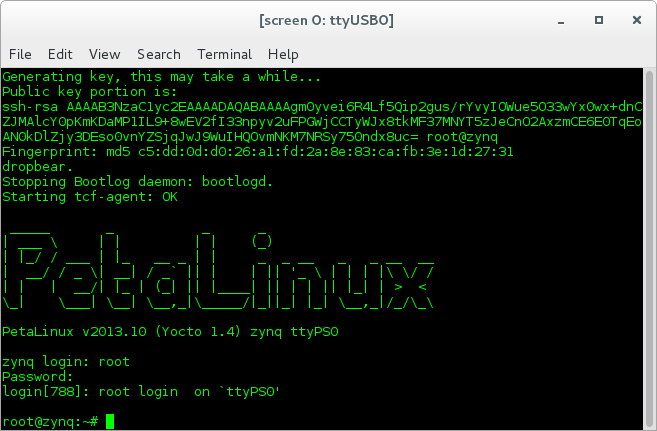
\includegraphics[scale=0.5]{Matchstiq_Z1_login}}
	\caption{Successful Boot}
	\label{fig:boot1}
\end{figure}
\subsubsection*{Using the Matchstiq-Z1 in Network Mode}
\begin{flushleft}
Every time the SDR is rebooted, the user is required to run the \texttt{mynetsetup.sh} script, which configures the system for OpenCPI with support for network/NFS mode\footnote{This script calls the \texttt{zynq\_net\_setup.sh} script, which is not user-modifiable.}. The user passes the network address of the development system in as the only argument to \texttt{mynetsetup.sh}.
\end{flushleft}
\begin{flushleft}
After the SDR is booted, the first thing that needs to be done is to source the \texttt{mynetsetup.sh} script with\\
\leavevmode{\parindent=3em\indent}\code{source /mnt/card/opencpi/mynetsetup.sh XX.XX.XX.XX}\\
and changing XX.XX.XX.XX to the IP address of the NFS host (your development machine, \textit{e.g.} 192.168.1.10). A successful run is shown in Figure~\ref{fig:netsetup}.
\end{flushleft}

\begin{figure}[H]
	\centerline{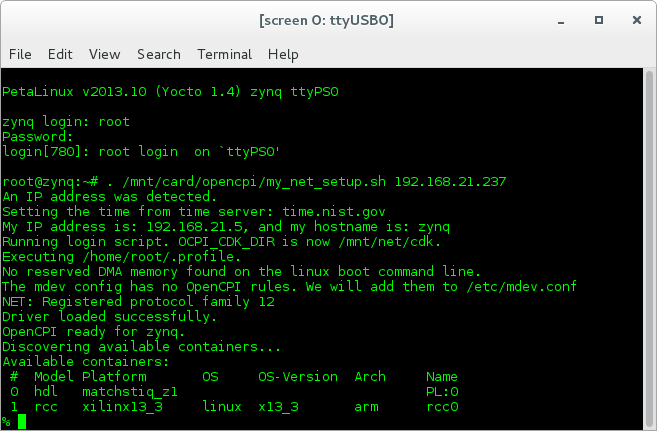
\includegraphics[scale=0.5]{Matchstiq_Z1_net_setup}}
	\caption{Successful Network Mode Setup}
	\label{fig:netsetup}
\end{figure}

\subsection{Standalone Mode}
All artifacts for any applications or tests that need to be located on the SD card must be on the ATLAS partition in the \texttt{opencpi/artifacts} folder.  All of the helper utilities such as \texttt{ocpirun} and \texttt{ocpihdl} are already located on the SD card and do not need to be copied over to the SDR platform.

\subsubsection*{Power cycle the Matchstiq-Z1}
The SDR should now boot a valid OpenCPI environment.  The user name and password for the SDR are both ``root''.  A successful boot up screen will look as follows:

\begin{figure}[ht]
	\centerline{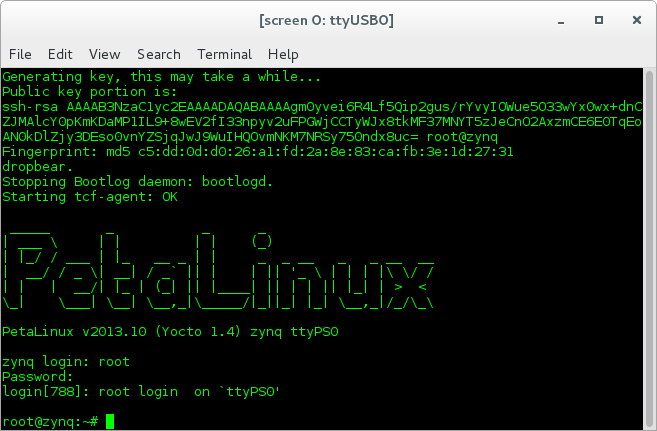
\includegraphics[scale=0.5]{Matchstiq_Z1_login}}
	\caption{Successful Boot}
	\label{fig:boot2}
\end{figure}

\subsubsection*{Using the Matchstiq-Z1 in Standalone Mode}
\begin{flushleft}
Every time the SDR is rebooted, the user is required to run the \texttt{mysetup.sh}, which configures the system for OpenCPI\footnote{This script calls the \texttt{zynq\_setup.sh} script, which is not user-modifiable.}. Any time that a new version of OpenCPI is released, the SD card will need to be recreated in order to update the artifacts and the executables that are stored on the SD card.
\end{flushleft}
\begin{flushleft}
After the SDR is booted, the first thing that needs to be done is to source the \texttt{mysetup.sh} script with\\
\leavevmode{\parindent=3em\indent}\code{source /mnt/card/opencpi/mysetup.sh}\\
A successful run of this will be as follows:
\end{flushleft}

\begin{figure}[ht]
	\centerline{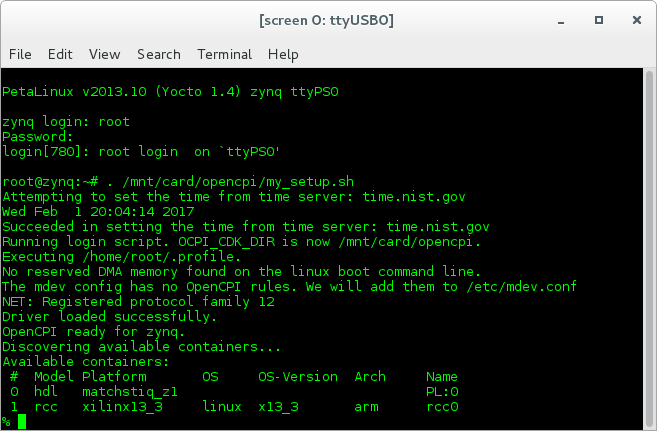
\includegraphics[scale=0.5]{Matchstiq_Z1_setup}}
	\caption{Successful Standalone Mode Setup}
	\label{fig:standalonesetup}
\end{figure}

\section{Verification}
The installation can be verified by running an application that uses both RCC and HDL workers.  There is an application that uses two RCC and one HDL worker located in \texttt{<Assets Project>/applications/bias.xml}. The two RCC workers are provided pre-built on the SD card or mounted CDK directory.  The HDL worker needs to be built into an assembly before the application can be executed.
\subsection{Building}
\label{sec:buildverify}
If operating in Standalone Mode, these steps should have been performed earlier. (See \ref{sec:buildNow}.)
\\ \\
First the Core project needs to be built for the matchstiq\_z1 platform.  This is performed at the top level of the Core project running the command \code{ ocpidev build -\--hdl-platform matchstiq\_z1}.  This will take about  45 minutes to complete.    
\\ \\
Then the matchstiq\_z1 platform needs to be built this is located in the Assets project.  To build this at the top level of the Assets project run the command \code{ocpidev build hdl platforms -\--hdl-platform matchstiq\_z1}.  This will take about 45 minutes to complete.
\\ \\
There is an existing assembly in the Assets Project that is the bias worker with its inputs and outputs connected to software.  This assembly needs to be built for ``matchstiq\_z1'' platform. It is located in \path{<Assets_Project>/hdl/assemblies/testbias/}.  At the top level of the project run the following command: ``\texttt{ocpidev build hdl assembly testbias -\--hdl-platform matchstiq\_z1}''.  This should take about 15 minutes to complete. You can confirm that it succeeded by locating the \texttt{*.bit.gz} file in \path{container-testbias_matchstiq_z1_base/target-matchstiq_z1/}.\\

\subsection{Running Network Mode}
The default setup script should already set the \texttt{OCPI\_LIBRARY\_PATH} variable to point to the RCC workers that are required to execute the application, but it needs to be updated to point to the assembly that was built.  After running the \texttt{mynetsetup.sh} script, navigate to  \texttt{/mnt/ocpi\_assets/applications}. Update the \texttt{OCPI\_LIBRARY\_PATH} variable using the following command: \\ ``\texttt{export OCPI\_LIBRARY\_PATH=\$OCPI\_LIBRARY\_PATH:/mnt/ocpi\_assets/hdl/assemblies/}''
In order to run the application, use the following command: ``\texttt{ocpirun -v -t 1 -d -m bias=hdl bias.xml}'' The output should be similar to Figure~\ref{fig:netBias}:
\begin{figure}[H]
	\centerline{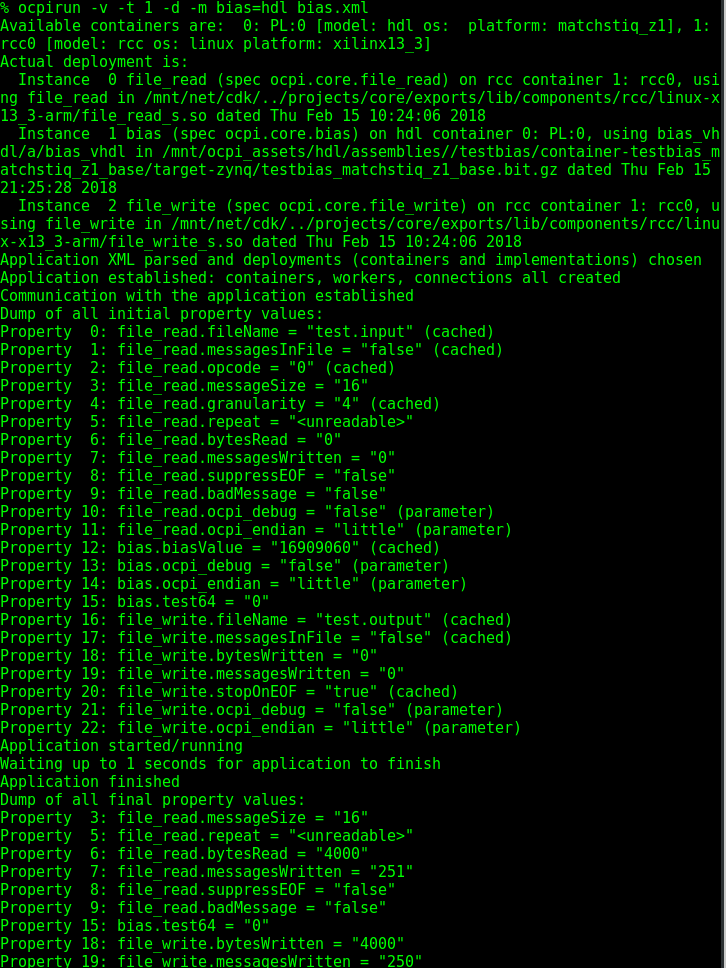
\includegraphics[scale=0.5]{Matchstiq_Z1_net_bias}}
	\caption{Successful Network Mode Execution}
	\label{fig:netBias}
\end{figure}

\begin{minipage}{\linewidth}
To view the input file, run the following command: ``\code{hexdump test.input | less}'' and the file should look like Figure~\ref{fig:inBias1}: \\ \medskip
\begin{figure}[H]
	\centerline{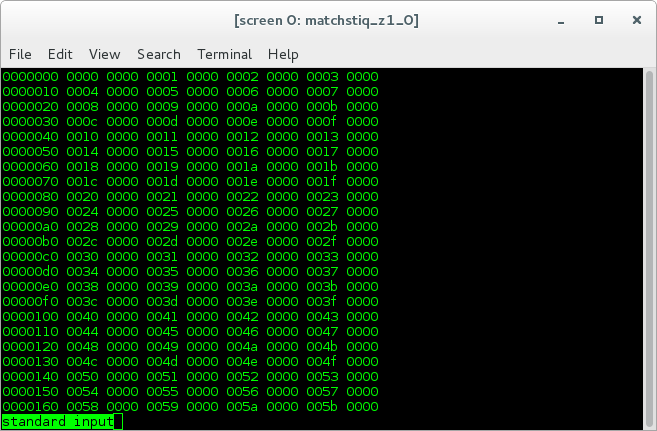
\includegraphics[scale=0.5]{Matchstiq_Z1_bias_input}}
	\caption{Expected Input}
	\label{fig:inBias1}
\end{figure}
\end{minipage}
~\\

\begin{minipage}{\linewidth}
To view the output file, run the following command: ``\code{hexdump test.output | less}'' and the file should look like Figure~\ref{fig:outBias1}: \\
\begin{figure}[H]
	\centerline{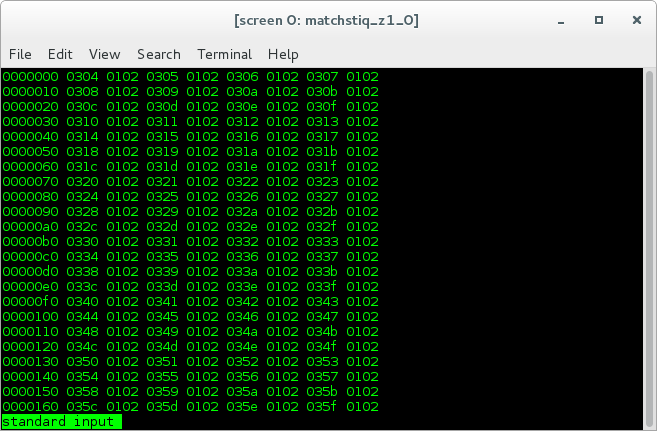
\includegraphics[scale=0.5]{Matchstiq_Z1_bias_output}}
	\caption{Expected Output}
	\label{fig:outBias1}
\end{figure}
\end{minipage}
~\\
\newpage
\subsection{Running Standalone Mode}
\begin{flushleft}
The default setup script should already set the \texttt{OCPI\_LIBRARY\_PATH} variable to all the required locations for the framework to execute the application.  All three of the artifacts that are located on the SD card are mounted at \texttt{/mnt/card/opencpi/artifacts}.  After running \texttt{mysetup.sh}, navigate to \texttt{/mnt/card/opencpi/xml}.  In order to run the application, use the following command: ``\code{ocpirun -v -t 1 -d -m bias=hdl bias.xml}'' The output should be similar to Figure~\ref{fig:standBias}:
\end{flushleft}
\begin{minipage}{\linewidth}
\begin{figure}[H]
	\centerline{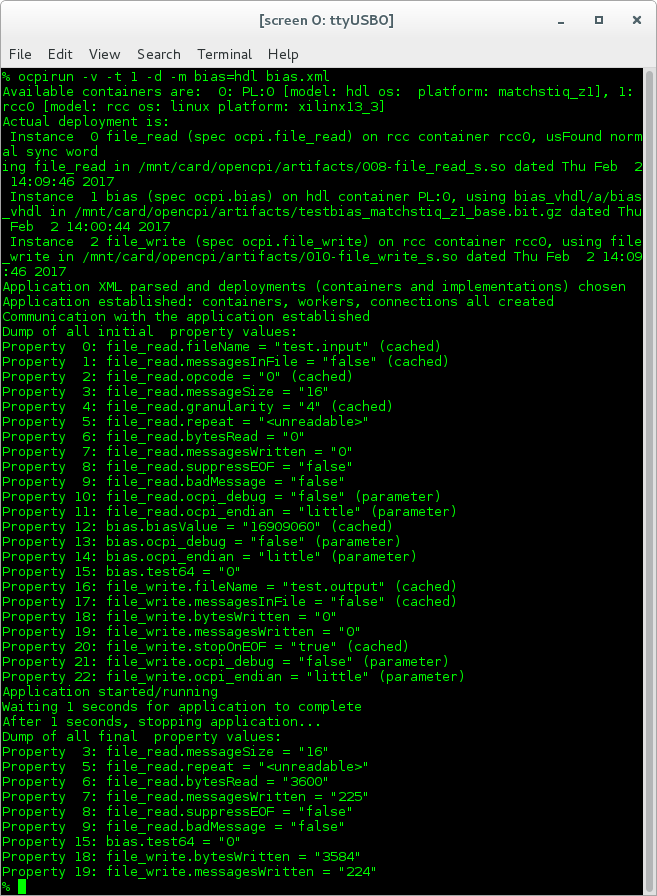
\includegraphics[scale=0.5]{Matchstiq_Z1_stand_bias}}
	\caption{Successful Standalone Mode Execution}
 \label{fig:standBias}
\end{figure}
\end{minipage}
~\\
\begin{minipage}{\linewidth}
To view the input file, run the following command: ``\code{hexdump test.input | less}'' and the file should look like Figure~\ref{fig:inBias2}: \\ \medskip
\begin{figure}[H]
	\centerline{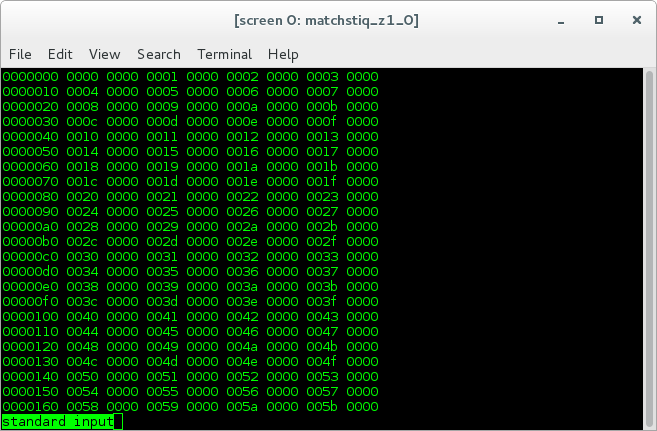
\includegraphics[scale=0.5]{Matchstiq_Z1_bias_input}}
	\caption{Expected Input}
	\label{fig:inBias2}
\end{figure}
\end{minipage}
~\\

\begin{minipage}{\linewidth}
To view the output file, run the following command: ``\code{hexdump test.output | less}'' and the file should look like Figure~\ref{fig:outBias2}: \\
\begin{figure}[H]
	\centerline{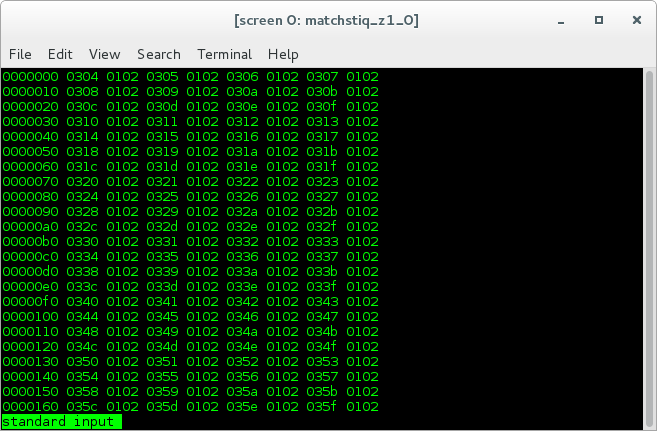
\includegraphics[scale=0.5]{Matchstiq_Z1_bias_output}}
	\caption{Expected Output}
	\label{fig:outBias2}
\end{figure}
\end{minipage}
~\\

\begin{appendices}
\section{Intermittent Errors}
Some tests have had ``Segmentation Faults'' or ``Alignment Errors'' in certain scenarios on the Z1. This seems to happen when both USB ports are used to simultaneously transmit a large amount of data, \textit{e.g.} high log-level output to a USB serial console as well as NFS-mounted output files over a USB-to-Ethernet adapter. The default test setup avoids triggering this by limiting output that is fed to the user, but users should be aware of this issue if non-default test scenarios are attempted. If \texttt{ssh} is used to have all data routed through the USB-to-Ethernet adapter, this failure mode is avoided.
\section{Using ISE instead of Vivado with the Matchstiq-Z1}
It is recommended that you use the default toolset (Xilinx Vivado) to build Matchstiq-Z1 bitstreams with OpenCPI. However, if you wish to use ISE instead, reference the README file in \path{<ocpiassets>/hdl/platforms/matchstiq_z1/}, and perform the following steps:
\begin{enumerate}
\item{Modify the target part in \path{<ocpiassets>/hdl/platforms/matchstiq_z1/matchstiq_z1.mk} to use the ISE alias:
\subitem \code{HdlPart\_matchstiq\_z1=xc7z\_ise\_alias\_020-1-clg484}}
\item{Export the ISE constraints files found in \path{<ocpiassets/>hdl/platforms/matchstiq_z1/ise_constraints/} by modifying \code{ExportFiles} variable in \path{<ocpiassets>/hdl/platforms/matchstiq_z1/Makefile}:
\subitem \code{ExportFiles=ise\_constraints/matchstiq\_z1.ucf ise\_constraints/matchstiq\_z1.ut matchstiq\_z1.mk}}
\end{enumerate}
% Bring in the kernel message snippet
\section{Driver Notes}
\input{../../../../../../doc/av/tex/snippets/Driver_Snippet.tex}
%

\end{appendices}
\end{document}
